% Options for packages loaded elsewhere
\PassOptionsToPackage{unicode}{hyperref}
\PassOptionsToPackage{hyphens}{url}
%
\documentclass[10pt,a4paper]{article}
\usepackage[left=25mm,right=25mm]{geometry}
\usepackage{amsmath}
\usepackage{amsfonts}
\usepackage{amssymb}

\author{}
\date{}



\usepackage{listings}
\usepackage{color}

\definecolor{dkgreen}{rgb}{0,0.6,0}
\definecolor{gray}{rgb}{0.5,0.5,0.5}
\definecolor{mauve}{rgb}{0.58,0,0.82}

\lstset{frame=tb,
  language=C,
  aboveskip=3mm,
  belowskip=3mm,
  showstringspaces=false,
  columns=flexible,
  basicstyle={\small\ttfamily},
  numbers=none,
  numberstyle=\tiny\color{gray},
  keywordstyle=\color{blue},
  commentstyle=\color{dkgreen},
  stringstyle=\color{mauve},
  breaklines=true,
  breakatwhitespace=true,
  tabsize=3
}

\usepackage{multicol}
\usepackage{graphicx}
\usepackage{epstopdf}

\epstopdfDeclareGraphicsRule{.gif}{png}{.png}{convert gif:#1 png:\OutputFile}
\AppendGraphicsExtensions{.gif}
\usepackage{chngcntr}
\counterwithin*{equation}{section}
\counterwithin*{equation}{subsection}
\usepackage{amsmath}

\usepackage{float} 
\usepackage{hyperref}
\usepackage{amsmath}
\let\oldsubsection\subsection
\renewcommand{\subsection}{%
    \setcounter{equation}{0}%
    \oldsubsection%
}
\begin{document}


\begin{flushleft}
\begin{LARGE}EE 435 Lab 2 Spring 2024
\end{LARGE}
\\Jonathan Hess and Grant Nordling
\\\href{https://github.com/Jetsama/EE435/tree/main/Labs/Lab2}{GitHub Page}
\end{flushleft}

\begin{LARGE}
Operational Amplifier Design
\end{LARGE}


The operational amplifier is one of the most widely used analog circuits with
virtually all analog and mixed-signal circuit designers being expected to be
knowledgeable about both the design and operation of the operational amplifier.
Although the concept of the operational amplifier is very fundamental and although there
have been a very large number of operational amplifiers designed by a large number of
engineers, the design of operational amplifiers continually presents challenges even to
experienced designers.
In this experiment, emphasis will be placed on the design of the most basic
operational amplifier, a single-stage amplifier with differential inputs and a single-ended
output using a tail-current bias. This basic structure can be systematically derived from
either an n-channel or a p-channel quarter circuit. The structure of this amplifier, based
upon the n-channel quarter circuit is shown in Fig. 1 where the transistor M9 has been
used to generate the tail-current bias.

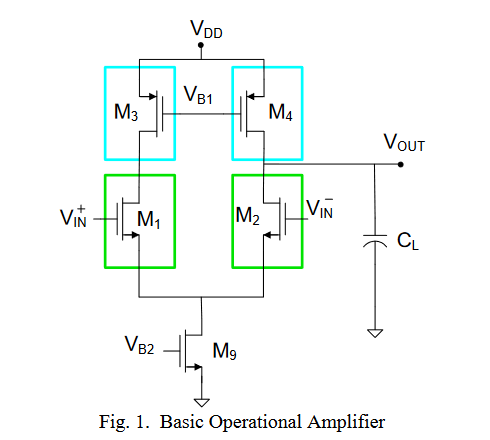
\includegraphics[width=3in]{images/figure1.png} \\
Although this circuit will work fine for the appropriate value of bias voltage VB1,
a common-mode feedback circuit (CMFB) is generally required to generate this bias
voltage and there is modest circuit overhead associated with the CMFB biasing circuit.
These will be discussed later in the course.
Since only a single-ended output is being used on this circuit, the voltage on the
drain node of M1 is not critical and it can be shown that this node can be used to bias M3
and M4 without requiring a CMFB. The modified version of this amplifier is shown in
Fig. 2 where the gates of M3 and M4 are connected so as to form a current mirror of the
current in M3 to that in M4

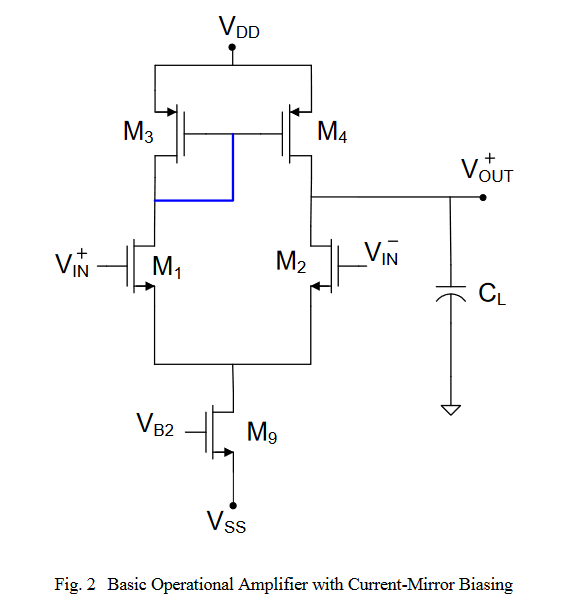
\includegraphics[width=3in]{images/figure2.png} \\

Fig. 2 where the gates of M3 and M4 are connected so as to form a current mirror of the
current in M3 to that in M4.
.VDD
M1 M2
VB2
M3 M4
VIN VIN
CL
M9
VOUT
VSS
Fig. 2 Basic Operational Amplifier with Current-Mirror Biasing
Our goal in this experiment will be to design an operational amplifier based upon
this architecture and to compare the theoretical values for some of the key performance
parameters of this structure with that obtained in a theoretical analysis. In this design, it
will be assumed that the TSMC 0.18$\mu$ CMOS process is to be used, the supply voltages
VDD and VSS are fixed at +1V and -1V respectively, the bias voltage VB2 is fixed at
-0.3V, and the capacitor CL is given. It will be assumed that the quiescent input voltages
are both 0V and the desired quiescent output voltage is also 0V though the amplifier can
be operated over some range of common-mode input and quiescent output values.
Consistent with the concept of symmetric circuits, it will be assumed that the circuit
will be designed under the assumption that matching between the left-half and the right-
half circuits is to be maintained.




\subsection*{Part 1}
Determine the number of degrees of freedom in this design and list the design
variables.\\

There are three degrees of freedom. We know with the traditional 4 transistor op amp we have four degrees. Now we after removing the need to bias the transistors 3 and 4 with a common mode feedback circuit, we also remove one parameter (and freedom) from the design.



\subsection*{Part 2}
Design an operational amplifier using the architecture of Fig. 2 that can drive a
capacitive load of 10pF using an analytical formulation for the amplifier. This design
should result in determining all of the natural design parameters for this circuit. The
amplifier should have a GB of at least 10MHz , a dc voltage gain of at least 100 when
driving this load, and a p-p output swing of 0.5V for some common-mode input levels
and some quiescent output level.\\

Using the following equations given in the lecture slides we can set our constraints. 
\begin{figure}[H]
\centering
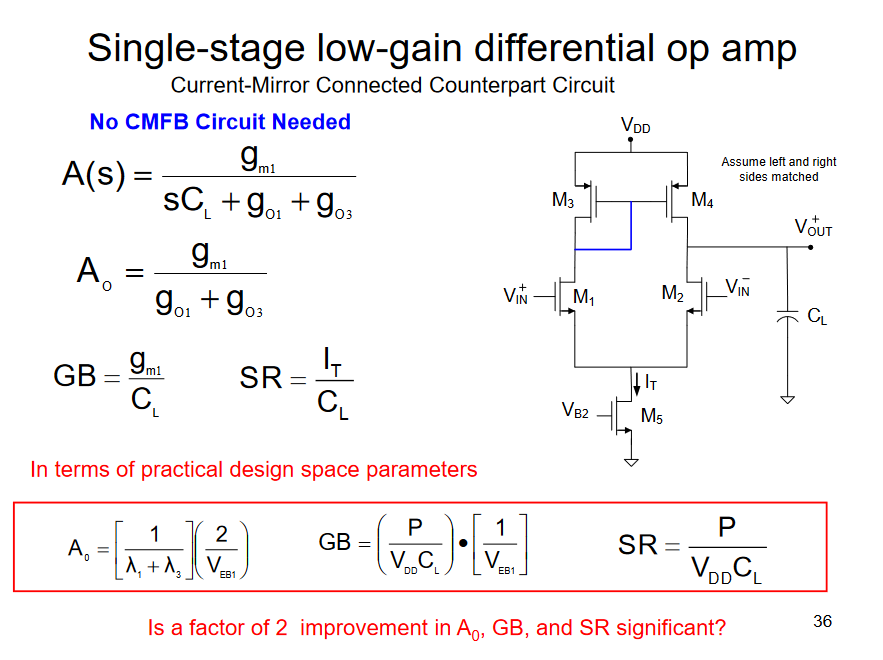
\includegraphics[width=3in]{images/diffopamp.png} \\
\caption{EE435 Lecture 5 Slide 36\cite{opamp}}
\end{figure}


The first step was setting the gain to 100. This requires finding the $\lambda_1$ and $\lambda_2$ (the channel-length modulation parameter). It is defined as the following.

To find the value the following testbench was created.
\begin{figure}[H]
\centering
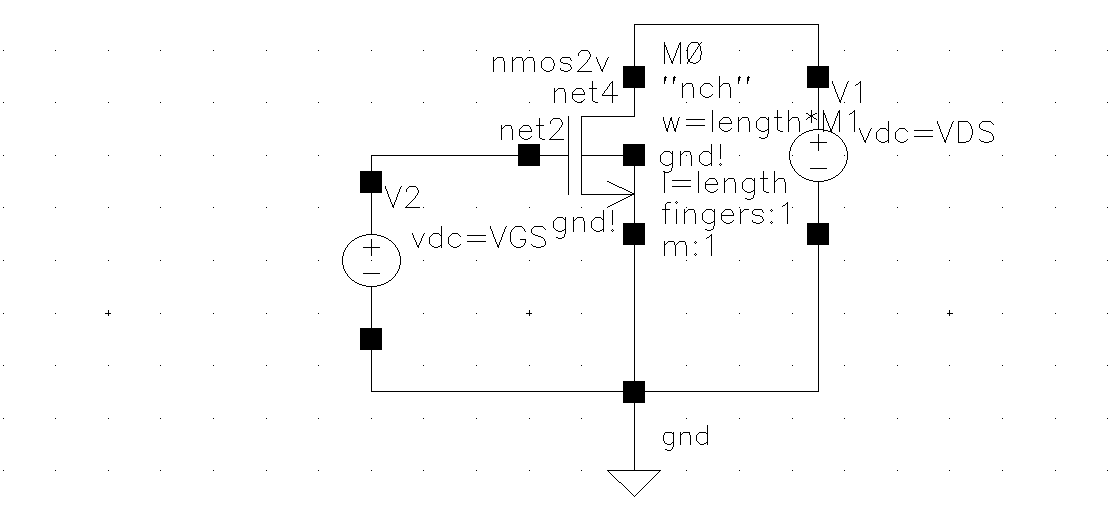
\includegraphics[width=3in]{images/mosTB.png} \\
\caption{EE435 Lecture 5 Slide 36\cite{opamp}}
\end{figure}

\begin{figure}[H]
\centering
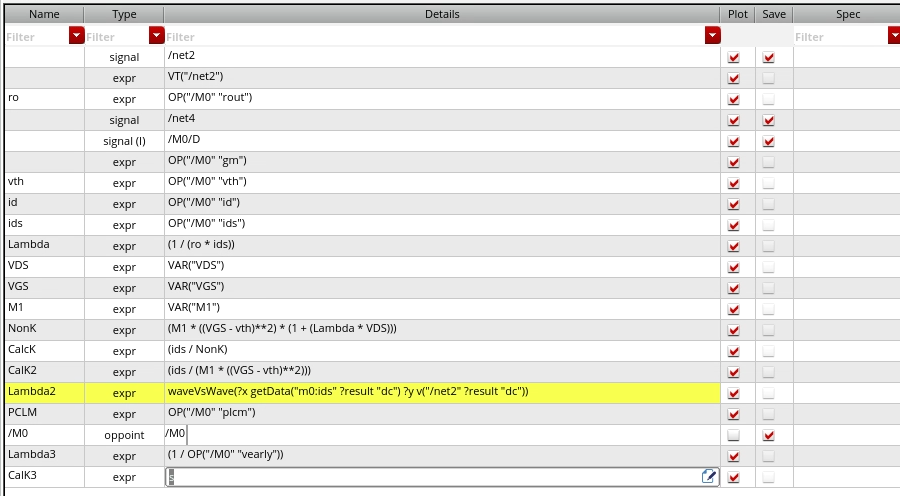
\includegraphics[width=6in]{images/mosTBEQ.png} \\
\caption{EE435 Lecture 5 Slide 36\cite{opamp}}
\end{figure}


\begin{figure}[H]
\centering
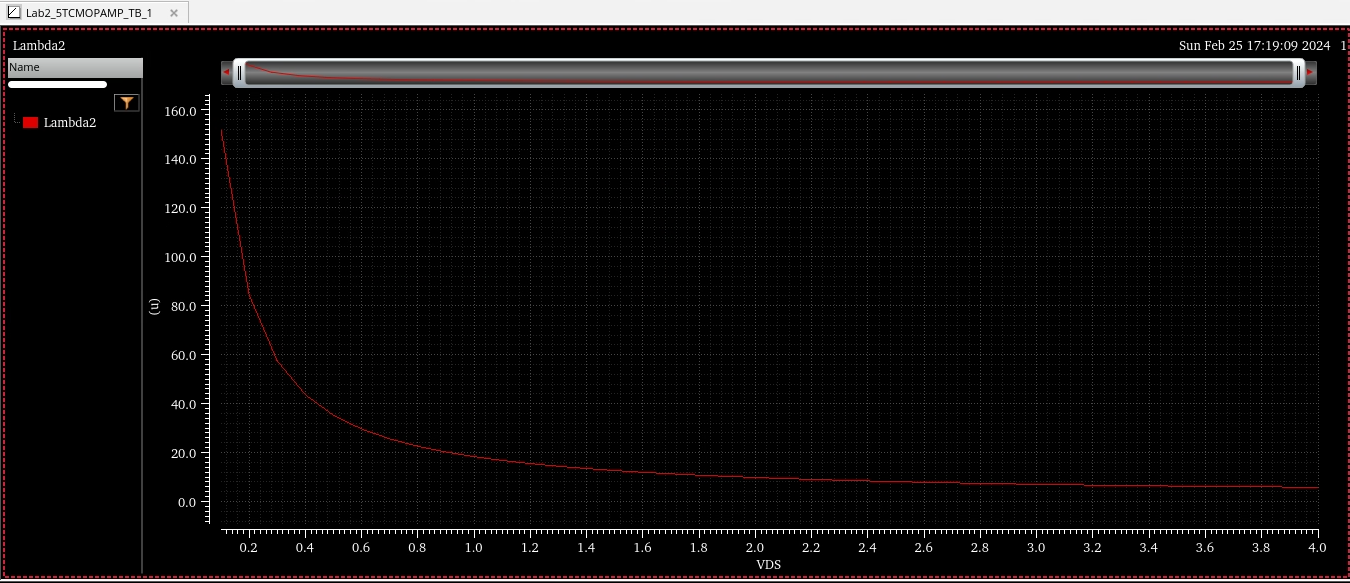
\includegraphics[width=6in]{images/lambda2graph.png} \\
\caption{EE435 Lecture 5 Slide 36\cite{opamp}}
\end{figure}

\subsection*{Part 3}
Simulate the amplifier you designed in Part 2 in Specrtre using the TSMC 0.18$\mu$
CMOS process. Compare the dc gain, the GB, the output signal swing, and the SR with
what you obtained by the analytical formulation.\\




\subsection*{Part 4}
Make minor changes, if necessary, in the design so that the simulated
performance meets the design requirements. Verify by computer simulations that the
performance requirements have been met.



\subsection*{Part 5}
Layout the circuit that you have designed and compare the post-layout extracted
performance with that of your circuit schematic. Resolve the reasons for any
discrepancies between the original schematic simulation and that of the extracted circuit.


\end{document}